\section{\scshape Results}\label{sec:results}

\subsection*{Results Overview}
\begin{frame}{Results Overview}
	\begin{table}[ht]
		\caption{Selection of the configurations with the best recognition results (1 configuration per image)}
		\centering
		\small
		\begin{tabu} { X[0.6,c,m] X[0.8,c,m] X[c,m] X[c,m] X[c,m] }
			\rowfont{\bfseries\itshape} Detector & Descriptor & Images with 1 banknote & Images with 2 banknotes & Images with 3 banknotes \\
			\noalign{\vskip 2mm} 
			\hline
			\noalign{\vskip 2mm} 
			SIFT	 & SIFT		  & 37			   & 7				  & 2	\\
			SURF	 & SURF		  & 24			   & 3				  & 0	\\
			GFTT	 & SIFT		  & 3			   & 1				  & 0	\\
			FAST	 & SIFT		  & 1			   & 0				  & 0	\\
			BRISK	 & BRISK	  & 1			   & 0				  & 0	\\
			ORB		 & ORB		  & 1			   & 0				  & 0	\\
		\end{tabu}
		\label{tab:recognition-configurations}
	\end{table}
\end{frame}


\subsection*{Front View Recognition With Clutter}
\begin{frame}{Front View Recognition With Clutter}
		\begin{figure}[H]
			\centering
			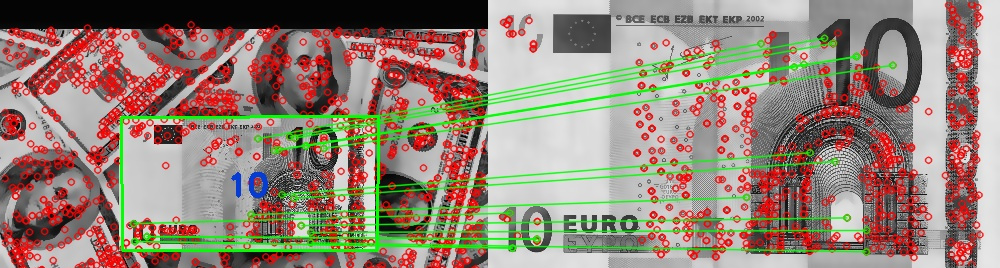
\includegraphics[width=\textwidth]{notes-recognition/10__(9).jpeg___SIFT-Detector_SIFT-Extractor_BF-Matcher_lowQualityImageDB_globalMatch__inliersMatches__0}
			\caption{Detection of a banknote in an ideal perspective view with background clutter (using SIFT detector, SIFT descriptors and BFMatcher)}
			\label{fig:recognition-clutter}
		\end{figure}
\end{frame}


\subsection*{Recognition With Perspective Distortion}
\begin{frame}{Recognition With Perspective Distortion}
	\begin{figure}[H]
		\centering
		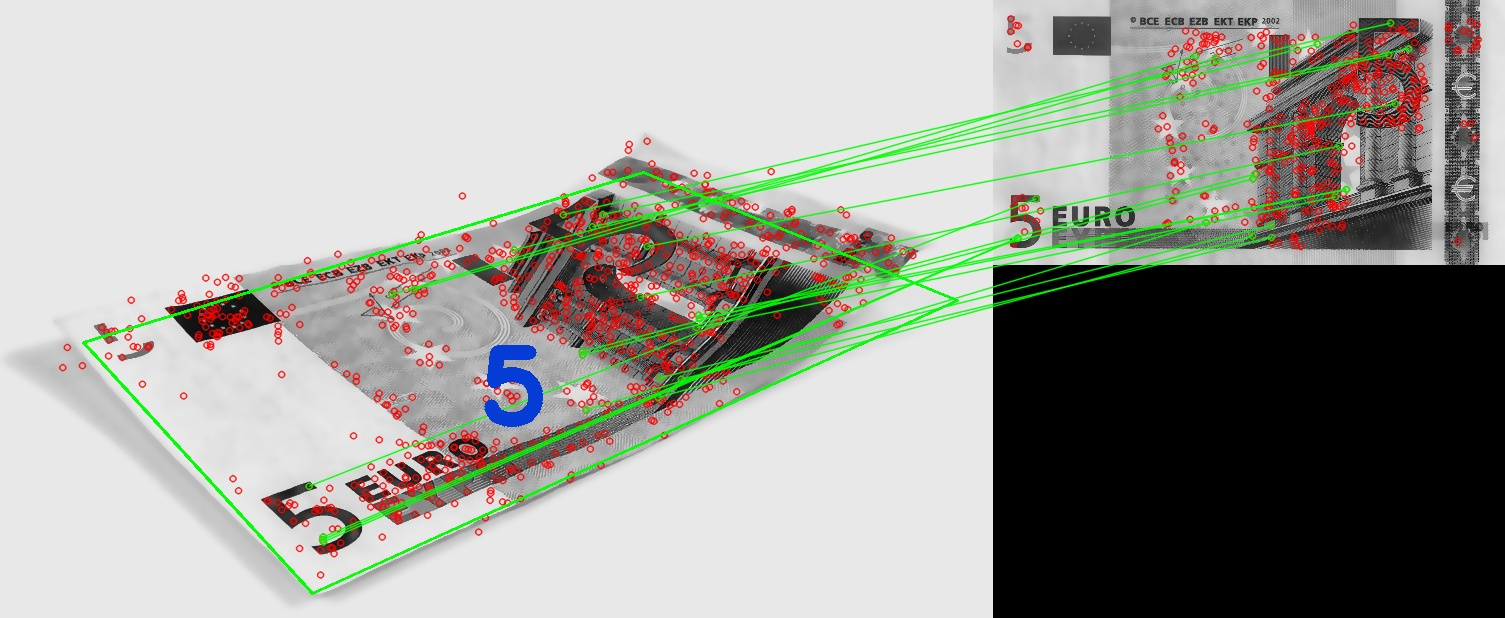
\includegraphics[width=\textwidth]{notes-recognition/5__(6).jpg___SURF-Detector_SURF-Extractor_BF-Matcher_lowQualityImageDB_globalMatch__inliersMatches__0}
		\caption{Detection of a banknote with perspective distortion and folding (using SURF detector, SURF descriptors and BFMatcher)}
		\label{fig:recognition-perspective-distortion}
	\end{figure}
\end{frame}


\subsection*{Recognition With Folding}
\begin{frame}{Recognition With Partial Folding}
	\begin{figure}[H]
		\centering
		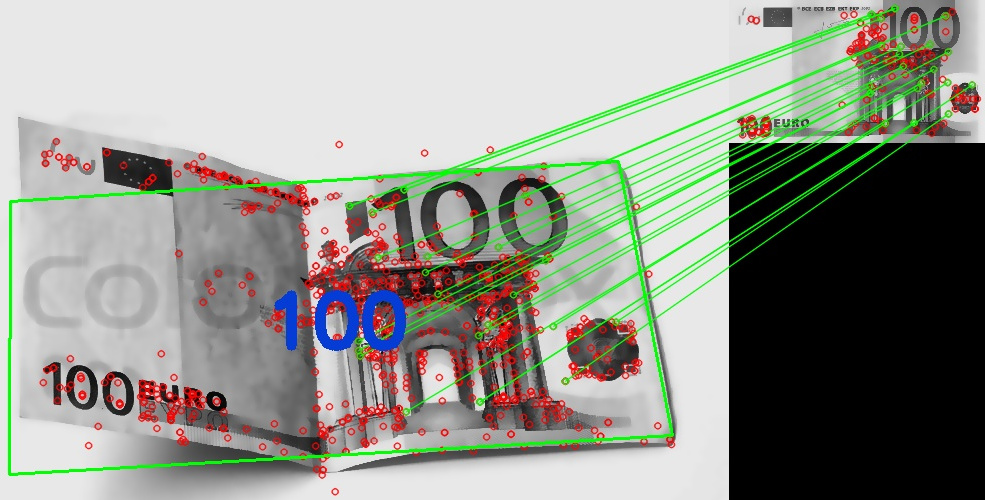
\includegraphics[width=\textwidth]{notes-recognition/100__(4).jpg___SIFT-Detector_SIFT-Extractor_BF-Matcher_dynamicQualityImageDB_globalMatch__inliersMatches__0.jpg}
		\caption{Detection of a partially folded banknote\\(using SIFT detector, SIFT descriptors and BFMatcher)}
		\label{fig:recognition-folding}
	\end{figure}
\end{frame}


\subsection*{Recognition With Occlusion}
\begin{frame}{Recognition With Occlusion}
	\begin{figure}[H]
		\centering
		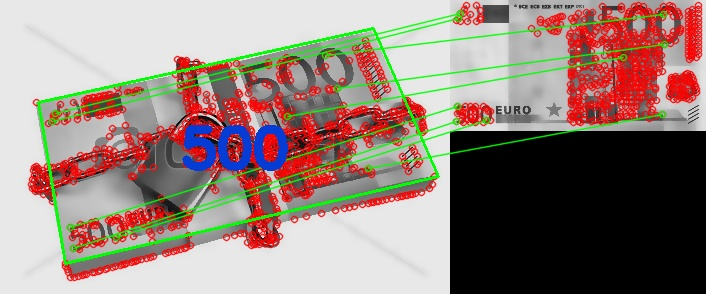
\includegraphics[width=\textwidth]{notes-recognition/500.jpg___GFTT-Detector_SIFT-Extractor_BF-Matcher_dynamicQualityImageDB_globalMatch__inliersMatches__0}
		\caption{Detection of a partially occluded banknote\\(using GFTT detector, SIFT descriptors and BFMatcher)}
		\label{fig:recognition-partially-occluded-banknotes}
	\end{figure}
\end{frame}


\subsection*{Recognition Of Partially Visible Banknotes}
\begin{frame}{Recognition of a Partially Visible Banknote}
	\begin{figure}[H]
		\centering
		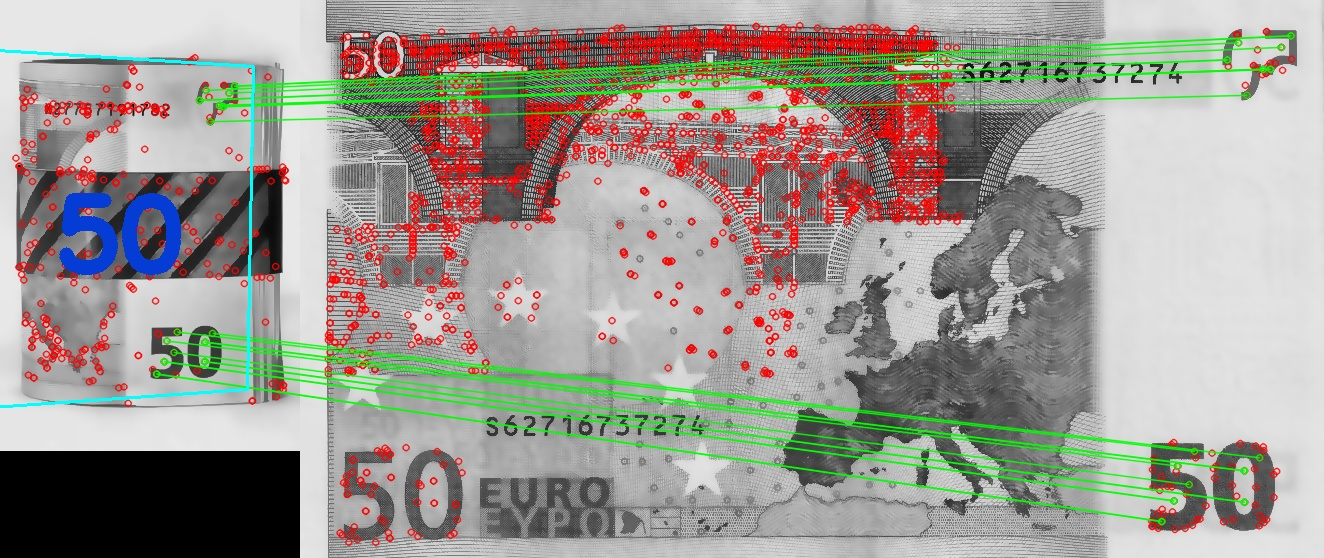
\includegraphics[width=\textwidth]{notes-recognition/50__(13).jpg___SIFT-Detector_SIFT-Extractor_BF-Matcher_mediumQualityImageDB_globalMatch__inliersMatches__0}
		\caption{Detection of a partially visible banknote\\(using SIFT detector, SIFT descriptors and BFMatcher)}
		\label{fig:recognition-partially-visible}
	\end{figure}
\end{frame}


\subsection*{Recognition Of Multiple Banknotes}
\begin{frame}{Recognition Of Multiple Banknotes}
	\begin{figure}[H]
		\centering
		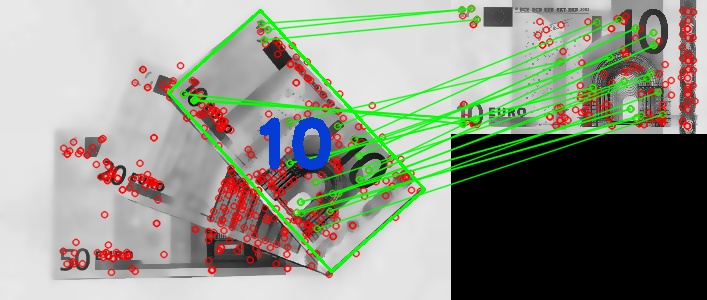
\includegraphics[width=\textwidth]{notes-recognition/10-20-50.jpg___SIFT-Detector_SIFT-Extractor_BF-Matcher_dynamicQualityImageDB_globalMatch__inliersMatches__1}
		\caption{Detection of the first overlapping banknote\\(using SIFT detector, SIFT descriptors and BFMatcher)}
		\label{fig:recognition-overlapping-banknotes-1}
	\end{figure}
\end{frame}

\subsection*{Recognition Of Multiple Banknotes}
\begin{frame}{Recognition Of Multiple Banknotes}
	\begin{figure}[H]
		\centering
		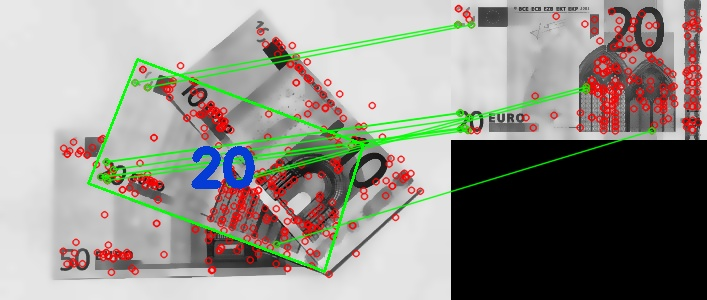
\includegraphics[width=\textwidth]{notes-recognition/10-20-50.jpg___SIFT-Detector_SIFT-Extractor_BF-Matcher_dynamicQualityImageDB_globalMatch__inliersMatches__2}
		\caption{Detection of the second overlapping banknote\\(using SIFT detector, SIFT descriptors and BFMatcher)}
		\label{fig:recognition-overlapping-banknotes-2}
	\end{figure}
\end{frame}

\subsection*{Recognition Of Multiple Banknotes}
\begin{frame}{Recognition Of Multiple Banknotes}
	\begin{figure}[H]
		\centering
		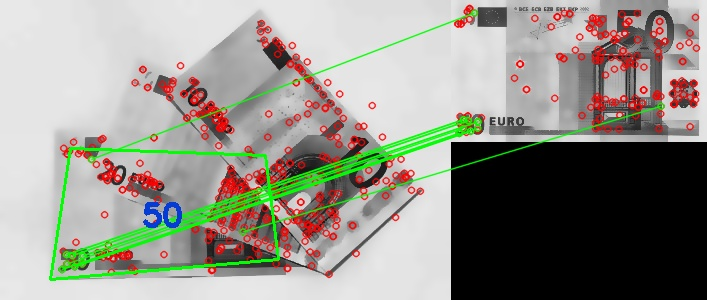
\includegraphics[width=\textwidth]{notes-recognition/10-20-50.jpg___SIFT-Detector_SIFT-Extractor_BF-Matcher_dynamicQualityImageDB_globalMatch__inliersMatches__0}
		\caption{Detection of the third overlapping banknote\\(using SIFT detector, SIFT descriptors and BFMatcher)}
		\label{fig:recognition-overlapping-banknotes-3}
	\end{figure}
\end{frame}


